\chapter{Aim of the Experiment, Theoretical Basis}
\section{Light in Quantum Mechanics}
The classical description of light as an electromagnetic field is given by the Maxwell equations. In Quantum Mechanics however, the electromagnetic field is treated differently. Here, it is based on the assumption, that every mode of the field corresponds to a harmonic oscillator. The Hamiltionian of a mode is 
\begin{equation}
    \hat{H}=\hbar \omega \left(\hat{n}+\frac{1}{2}\right)~.
\end{equation}
The electromagnetic field is treated as a quantized excitation of packages with the energy $\hbar \omega$, which are photons. In contrary to classical electrodynamics, in which the energy can attain arbitrary small energies, the energy in quantum mechanics are discrete with the photon being the smallest possible excitation of the field.

\section{Fock States}
Fock states are the fundamental excitations of the electromagnetic field and are the eigenstates $\ket{n}$ of the Hamiltonian $\hat{H}$ and the number operator $\hat{n}$. A single photon is the fundamental excitation quantum and therefore the smallest possible excitation of the electromagnetic field. It is described by the Fock state $\ket{1}$. When there are no photons, the field is in the ground state $\ket{0}$. This state is also called vacuum state. The number of photons $n$ that a field mode in a Fock state has are given by the expectation value
\begin{equation}
    \bra{n}\hat{n}\ket{n}=n 
\end{equation}
and the variance
\begin{equation}
    \Delta n^{2}=\bra{n}\hat{n}^{2}\ket{n}-\bra{n}\hat{n}\ket{n}^{2}=0~.
\end{equation}
\begin{figure}[H]
    \centering
    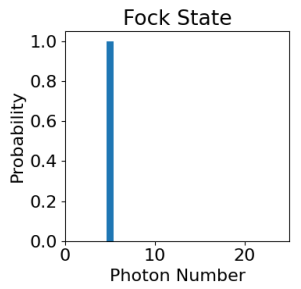
\includegraphics[width=50mm,scale=0.5]{Quantenoptik/include/Fock state.PNG}
    \caption{Photon number probability for a Fock state with $\braket{n}=5$} 
    \label{fig:Fock state}
\end{figure}


\section{Coherent States}
A laser emits plane electromagnetic waves with constant amplitudes. Such a plane wave is described by a coherent state $\ket{\alpha}$ which are a linear combination of Fock states \begin{equation}
    \ket{\alpha}=e^{-\frac{|\alpha|^{2}}{2}}\cdot \sum_{n=0}{\infty}\left(\frac{\alpha ^{n}}{\sqrt{n!}}\cdot \ket{n}\right)~.
\end{equation}
Coherent states are eigenstates of the annihilation operator $\hat{a}$. The expectation value of the number operator \begin{equation}
    \braket{n}=|\alpha|^{2}
\end{equation}
and the variance 
\begin{equation}
    \Delta n^{2}=\bra{n}\hat{n}^{2}\ket{n}-\bra{n}\hat{n}\ket{n}^{2}=|\alpha|^{2}
\end{equation}
are equal which hints that the photon numbers follow a Poisson distribution which can be seen in the figure 2.
\begin{figure}[H]
    \centering
    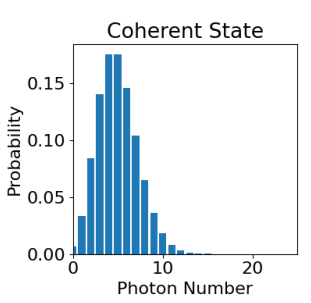
\includegraphics[width=50mm,scale=0.5]{Quantenoptik/include/Coherent state.PNG}
    \caption{Photon number probability for a Coherent state with $\braket{n}=5$} 
    \label{fig:Coherent state}
\end{figure}


\section{Thermal States}
Lights like the radiation emitted by a black body or LEDs are in chaotic states and are described by a statistical mixture of pure states. These chaotic lights are in thermal states and are described by the density matrix. The most prominent example is the black body 
\begin{equation}
    \hat{\rho}=\left(1-e^{-\frac{\hbar \omega}{k_\text{B} T}}\right) \cdot e^{-\frac{\hbar \omega \hat{n}}{k_\text{B} T}}~.
\end{equation}
The variance 
\begin{equation}
    \Delta n^{2}=\braket{n^{2}}-\braket{n}^{2}=\braket{n}^{2}+\braket{n}
\end{equation} is always larger than the expectation value and therefore larger than for a Poissonian distribution like coherent states.
\begin{figure}[H]
    \centering
    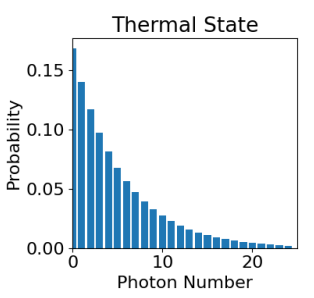
\includegraphics[width=50mm,scale=0.5]{Quantenoptik/include/Thermal state.PNG}
    \caption{Photon number probability for a Thermal state with $\braket{n}=5$} 
    \label{fig:Thermal state}
\end{figure}


\section{Second-Order Correlation Function}
To test the quantum nature of light, a simple experiment with an intensity interferometer, introduced by Hanbury, Brown and Twiss, can be done. In this experiment, a light beam with very low intensity is send through a beamsplitter with two detectors at the outputs. Due to the fact that light is quantized, a single quantum can only be detected at one of the detectors. \\
A quantity that can be measured with this setup is the second-order correlation function 
\begin{equation}
    g^{(2)}(\tau)=\frac{\braket{I_\text{A}(t+\tau)} \cdot I_\text{B}(t)}{\braket{I_\text{A}(t+\tau)} \cdot \braket{I_\text{B}(t)}}~.
    \label{eq:Cf}
\end{equation}
This function describes the correlation of the intensities $I_\text{A}, I_\text{B}$ that are detected at the detectors A and B at the times $t$ and $t+\tau$. The most important and the value of the function that is of interest in this following experiments, is the correlation of the detector signals for $\tau=0$, thus at the same time 
\begin{equation}
    g^{(2)}(0)=\frac{\braket{I_\text{A} \cdot I_\text{B}}}{\braket{I_\text{A}} \cdot \braket{I_\text{B}}}~.
\end{equation}
If $g^{(2)}(0)<1$, the detector signals are anit-correlated, which means that there is a high signal on one detector while the other detector  has a low signal. If $g^{(2)}(0)=1$, the signals are uncorrelated. If $g^{(2)}(0)>1$, the signals are correlated. In this case, one detector measures a large signal and the other also measures a large signal. \\
The expected value of $g^{(2)}(0)$ depend on the characteristics of the incoming light. To list a few examples, for a single photot $g_\text{HBT}^{(2)}(0)$ takes the value 1. Meaning the photon is only detected at one output of the beamsplitter. A strongly attenuated laser, which is described by coherent light ha a second-order correlation function equal to 1. For thermal light $g_\text{HBT}^{(2)}(0)=2$. This means, that the source emits no photons most of the time, but when it does, it emits multiple the same time with half of the photons being measured at the two detectors, respectively. It can be proven, that for classical fields, $g_\text{HBT}^{(2)}(0) \geq 1$. The beamsplitter splits the wave into two parts with constant ratio, hence there can be no anti-correlation of the signals.


\section{Correlation Function for Single Photon Detectors}
Single photon detectors are used to detect very low intensities. The outcomes of the detectors are not continuous signals, but single output pulses that are called clicks or counts. Equation \eqref{eq:Cf} can be modified to calculate the correlation function for single photon detectors using count rates instead of intensities. This yields 
\begin{equation}
    g^{(2)}(\tau)=\frac{R_\text{AB}(\tau)}{R_\text{A}\cdot R_\text{B}\cdot \Delta t}~.
\end{equation}
For $\tau=0$ 
\begin{equation}
    g^{(2)}(0)=\frac{R_\text{AB}}{R_\text{A}\cdot R_\text{B}\cdot \Delta t}
\end{equation}
with the count rates $R_\text{A}, T_\text{B}$ of the detectors A and B, the count rates of coincidences of $R_\text{AB}$ and the time window $\Delta t$.


\section{Spontaneous Parametric Down-Conversion}
\begin{figure}[H]
    \centering
    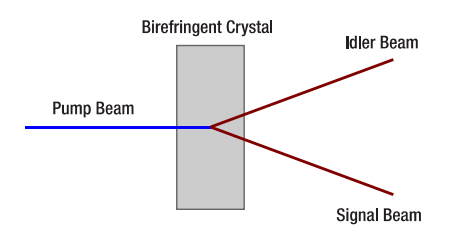
\includegraphics[width=70mm,scale=0.5]{Quantenoptik/include/crystal.PNG}
    \caption{Schematic drawing of the SPDC process} 
    \label{fig:SPDC}
\end{figure}
To obtain photon pairs, one can use a process called Spontaneous Parametric Down-Conversion (SPDC). Here, photon pairs are generated inside a nonlinear crystal from pump light. The photons of one pair are called "`idler"' and "`signal"' and are created virtually simultaneously. By that, one photon is used to signal the existence of the other. In SPDC processes, certain crystals are used. Under the assumption, that the idler and signal photons have similar wavelengths, the index of refraction for pump, idler and signal photons have to be the same. Therefore, birefringent crystals are used. Those crystals have different indices of refraction for different polarizations. 